\subsubsection{\stid{2.07} YTune} 

\paragraph{Overview}

We are developing tools and an application development workflow that separates a high-level C/C++/FORTRAN implementation from an architecture-specific implementation (OpenMP, CUDA, etc.), optimization, and  tuning.   This  approach
will enable Exascale application  developers to express and  maintain a
single, portable implementation of their computation that is also legal code
that can be compiled and run by using standard tools.   The autotuning compiler
and search framework will transform the baseline code into a   collection of
highly-optimized implementations. This reduces the need for extensive manual tuning.
Both code transformation and autotuning are essential in ECP for providing
performance portability on Exascale platforms.  Due to significant architectural
differences in ECP platforms, attaining performance portability may  require
fundamentally different  implementations of software -- different strategies for
parallelization, loop order,  data layout, and exploiting SIMD/SIMT.  A key
concern of ECP is the high cost of developing  and maintaining
performance-portable applications for  diverse Exascale architectures, including
manycore CPUs and GPUs. 
Ideally Exascale application developers would express their
computation separate from   its mapping to hardware, while autotuning compilers can automate this mapping and achieve performance portability.

\paragraph{Key  Challenges}
Autotuning has the potential to dramatically improve the performance portability of Petascale and Exascale applications.  To date, autotuning has been used primarily in high-performance applications through tunable libraries or previously tuned application code that is integrated directly into the application.
If autotuning is to be widely used in the HPC community,
support for autotuning must address the software engineering challenges, manage configuration overheads, and continue to demonstrate significant performance gains and portability across architectures.
In particular, tools that configure the application must be integrated into the application build process so that tuning can be reapplied as the application and target architectures evolve.

\paragraph{Solution Strategy}
We are developing pluggable software infrastructure that incorporates
autotuning at different levels: compiler optimization, runtime configuration of application-level parameters and system software.
To guarantee success in the ECP time frame, we are collaborating with
application teams, such as SuperLU and QMCPACK, to impact performance of their
codes and libraries.

The autotuning compiler strategy revolves CHiLL, which has the following distinguishing features:
(1) \textit{Composable transformation and code generation}, such
that the same tool can be applied
to multiple different application domains;
(2) \textit{Extensible to new domain-specific transformations} that can be represented as transformations on loop nest iteration spaces are also
composable with existing transformations;
(3) \textit{Optimization strategies and parameters exposed to autotuning:}
By exposing high-level expression
of the autotuning search space as transformation recipes, the compiler writer, an expert programmer or embedded DSL designer can directly \
express how to compose
 transformations that lead to different implementations.
A part of our efforts in ECP are to migrate these capabilities of CHiLL
into the Clang/LLVM open-source compiler, as well as provide lightweight
interfaces through Python, C++, and REST APIs/web services.

For example, we have developed a \textit{brick data layout library and code generator} for
stencil computations within CHiLL.
Recent trends in computer architecture that favor computation over data movement incentivize high-order methods.  Paradoxically, high-order codes can be challenging for compilers/optimization to attain high performance.  Bricks enable high performance and make fine-grained data reuse and memory access information known at compile time.  The SIMD code generation achieves performance portability
for high-order stencils for both CPUs with wide SIMD units (Intel Knights
Landing) and GPUs (NVIDIA Pascall).  Integration with autotuning attains
performance that is close to Roofline performance bound for both manycore CPU
and GPU architectures.

The Search using Random Forests (SuRF) search framework is a separate tool in Y-Tune that optimizes the search over an autotuning search space.  While
SuRF provides support to CHiLL for compiler-directed autotuning, it can
also be integrated directly with applications and runtimes to search over
application parameters and alternative code variants.
SuRF is an asynchronous search framework that consists of sampling a small number of input parameter configurations and progressively fitting a surrogate model over the input-output space until exhausting the user-defined maximum number of evaluations. The framework is designed to operate in the master-worker computational paradigm, where one master node fits the surrogate model and generates promising input configurations and worker nodes perform the computationally expensive evaluations and return the outputs to the master node. We implemented both MPI- and scheduler-based master-worker approaches.


\paragraph{Recent Progress}


We have pursued the following main activities since the beginning of 2018:

\textit{Autotuning capability in LLVM:}
The key idea is to support the use of pragmas in the C++ source to guide transformations to be applied. These can include the types of transformation recipes used in CHiLL, but also parallelization directives for OpenMP and OpenACC that would interact with SOLLVE and PROTEAS. Our initial focus is the implementation of user/tool-directed optimizations in Polly, which is a polyhedral framework in LLVM with some similar features to CHiLL. An initial plan for pragmas in Clang and LLVM metadata has been developed. Several existing open-source LLVM projects allowing for just-in-time (JIT) compilation of C++ code have been identified and are being evaluated for use with autotuning. A summer intern has been identified who will work on the JIT/autotuning explorations.

\vspace*{.1in}
\noindent
\textit{SuRF for SuperLU and QMCPACK:}
We focused on testing and hardening SuRF for tuning SuperLU package. We used 6 matrices that come from different DOE applications and ran SuRF in an asynchronous mode with up to 32 nodes. We compared the results from SuRF to those from OpenTuner. On all instances tested, we found that SuRF obtains comparable results but in half the time of OpenTuner. We also observed that SuRF found high quality solutions in short computation time and used the remaining time for neighborhood exploration. Therefore, we implemented early stopping criterion. We also did single node tuning experiments with QMC. Since the current search space of QMCPACK is rather small, we did not evaluate it at scale. Currently, we are working with the QMCPACK developers to expose more parameters.
Recently, we developed stopping criterion based on local convergence and expected improvement over time. This allows the search to terminate in shorter computation time. Currently, we are expanding the search for multinode autotuning where each evaluation spans multiple nodes.

\vspace*{.1in}
\noindent
\textit{Brick Library:}
We developed a code generator for the Brick Data Layout library for stencils
that is performance-portable across CPU and GPU architectures, and addresses the
needs of modern multi-stencil and high-order stencil computations. The key
components of our approach that lead to performance portability are (1) a
fine-grained brick data layout designed to exploit the inherent multidimensional
spatial locality common to stencil computations; (2) vector code generation that
can either target wide SIMD CPU instructions sets such as AVX-512 and SIMT
threads on GPUs; and, (3) integration with autotuning framework to apply
architecture-specific tuning. For a range of stencil computations, we show that
it achieves high performance for both the Intel Knights Landing (Xeon Phi) CPU,
and the NVIDIA P100 (Pascal) GPU \cite{P3HPC_Bricks}. 

\paragraph{Next Steps}
In the near future, we will release the CHiLL autotuning compiler, and
demonstrate application and library kernel performance gains from 
using the brick data layout.  We will continue the transition of CHiLL capabilities to LLVM.
In SuRF, we plan to explore multinode search, and integrate SuRF into the compiler-directed autotuning we are doing.

\begin{figure}[h]
%\begin{wrapfigure}{r}{0.35\textwidth}                                                                                                     
\begin{center}
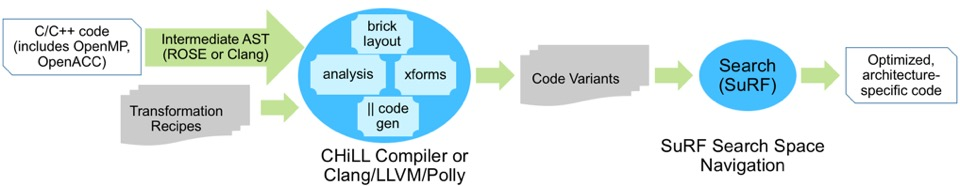
\includegraphics[width=.8\textwidth]{projects/2.3.2-Tools/2.3.2.07-Autotuning/YTune-solution.jpg}
% 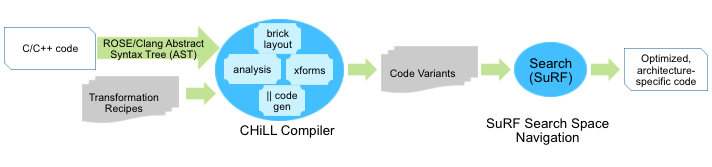
\includegraphics[width=.8\textwidth]{YTune-solution.png}
% \includegraphics[width=.8\textwidth]{PastedGraphic-1.png    }
\end{center}
\caption{Y-TUNE Solution Approach.}
%\caption{S.}                                                                                                                              
%\end{wrapfigure}                                                                                                                          
\end{figure}

%\end{document}
